\documentclass{beamer}

\usepackage{slides}
\usepackage{vwcol}
\usepackage{multicol}
\usepackage{gensymb}


\begin{document}

\title{Analysis of whistler weather data}
\author{Benjamin, Ethan and Nathan \\ \vspace{1mm}
Stat 300 Project, Fall 2015}
\date{December 2, 2015}

\begin{frame}
\titlepage
\end{frame}

\begin{frame}{Outline}

\color{black}{
\tableofcontents}
\end{frame}

\begin{frame}{Objectives}

\section{Background}

\begin{enumerate}
\item Determine start, peak and end of winter season
\item Determine how much snow is present at different points in year
\item Determine trends and odd behaviors in data
\end{enumerate}

\end{frame}

\begin{frame}{Background}

%\section{Data}

\begin{columns}

\column{0.32\textwidth}

{\small
\begin{itemize}
\item Whistler Blackcomb
\begin{itemize} 
\item Dependent on snow
\end{itemize}
\item Data
\begin{itemize}
\item Elevation: 650m
\item Precipitation and wind not used
\end{itemize}
\end{itemize}
}

\vspace{30mm}

\column{0.8\textwidth}

\vspace{-18mm}
\begin{figure}
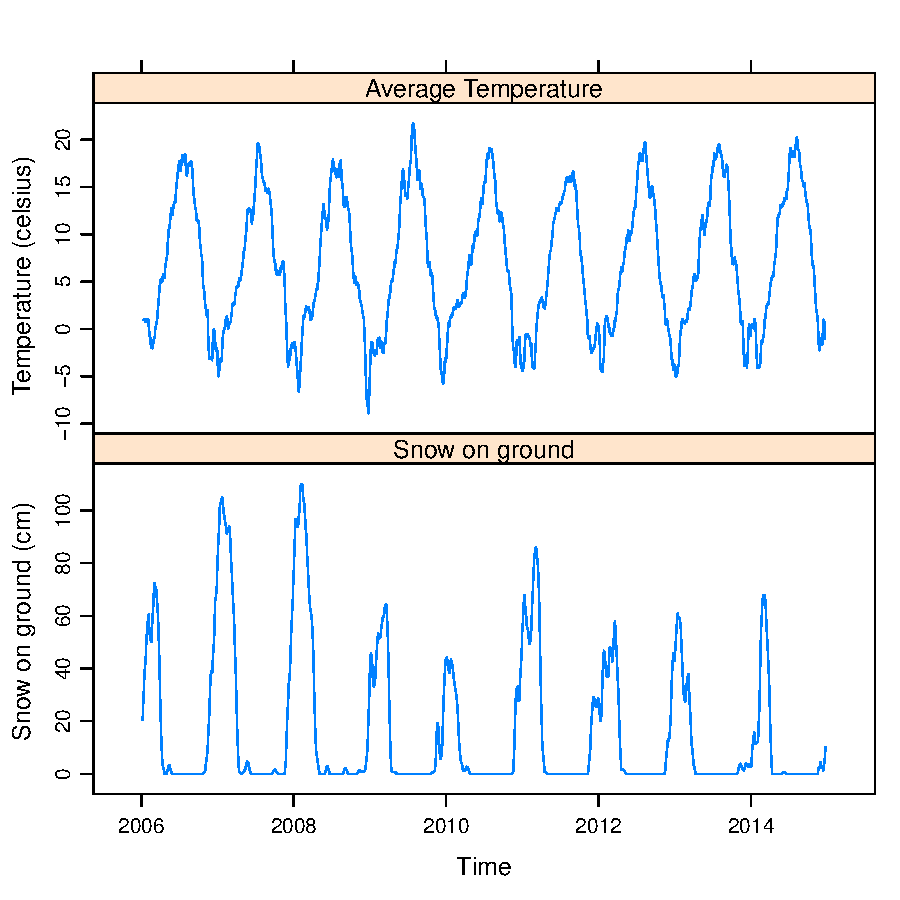
\includegraphics[width=0.9\textwidth]{report-basicts}
\vspace{-2mm}
\caption{{\footnotesize Whistler temperature and snowfall from 2006--2014}}
\vspace{10mm}
\end{figure}

\end{columns}

\end{frame}

\begin{frame}{Methods}

\section{Methods and Results}

\begin{itemize}

\item Exploratory
\item Statistical techniques 
\begin{enumerate}
\item Regression: trend
\item Time series techniques: compare different winter seasons
\item Correlation: relationship between temperature and snowfall
\end{enumerate}

\item Winter: period when one week moving average for snowfall was greater than 15 cm 
\end{itemize}

\end{frame}

\begin{frame}{Snowfall trend}

\subsection{Trend}

\begin{columns}

\column{0.3\textwidth}

{\small
\begin{itemize}
\item Linear regression
\item $p$-value $<$ 0.001
%\item Using trend for projection wouldn't be accurate (recent upward trend in peak snowfall)
\item Temperature trend is not as noticeable
\end{itemize}
}

\vspace{30mm}

\column{0.75\textwidth}

\vspace{-18mm}
\begin{figure}
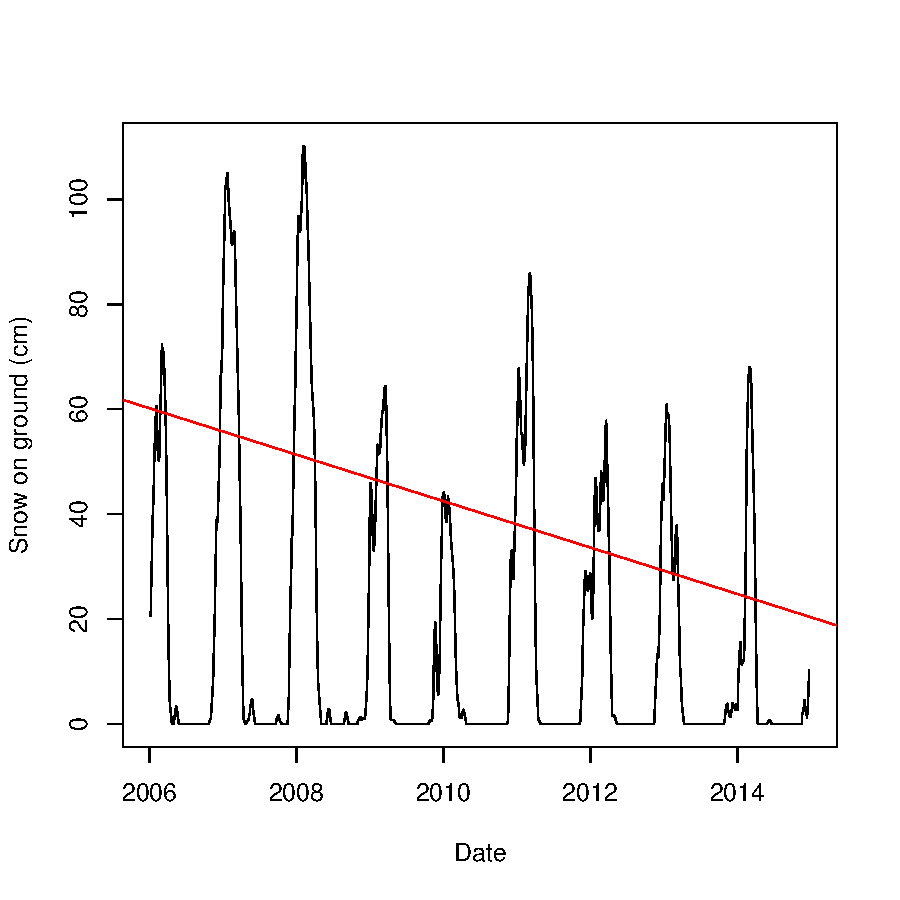
\includegraphics[width=0.9\textwidth]{report-snowtrend}
\vspace{-2mm}
\caption{{\footnotesize Downwards trend of 4.42 cm per year}}
\vspace{10mm}
\end{figure}

\end{columns}

\end{frame}

\begin{frame}{Average smoothing}

\subsection{Average smoothing}

\begin{columns}

\column{0.32\textwidth}

{\small
\begin{itemize}
\item Period shown is July 1 -- June 30
\item Maximum
\begin{itemize}
\item Snow all months except July, August
\end{itemize}
\item Minimum
\begin{itemize}
\item Snow from December to mid--April
\end{itemize}
\end{itemize}
}

\vspace{10mm}

\column{0.8\textwidth}

\vspace{-18mm}
\begin{figure}
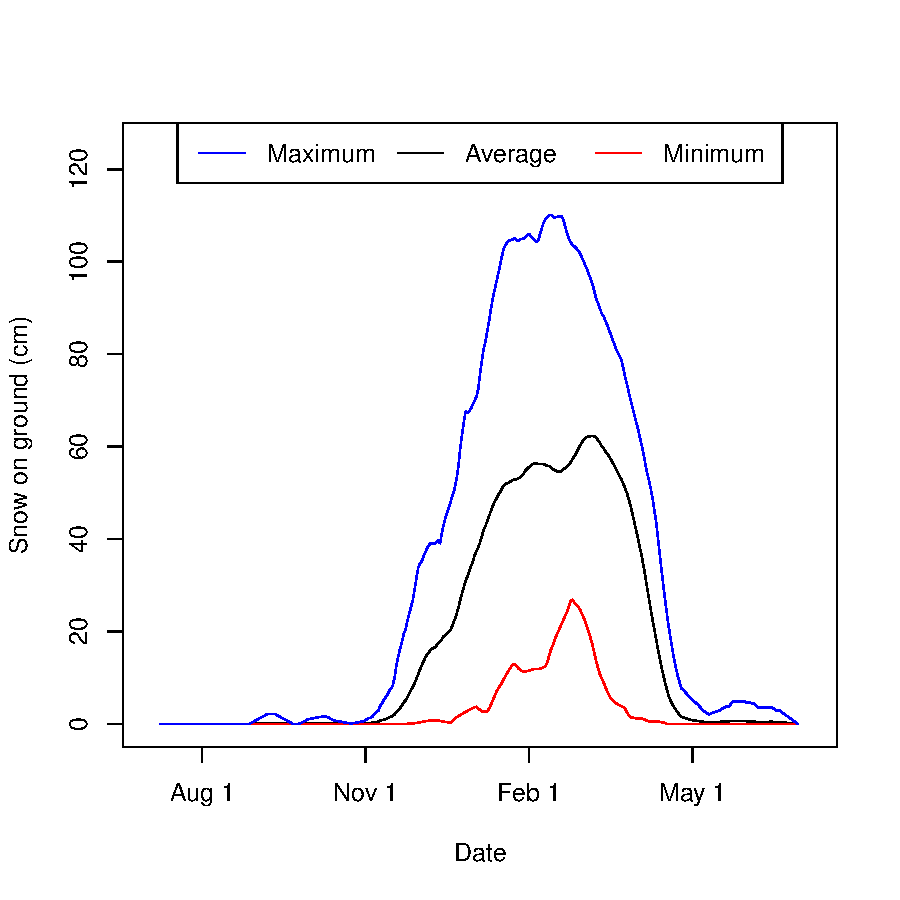
\includegraphics[width=0.9\textwidth]{report-averagetsplot}
\vspace{-2mm}
\caption{{\footnotesize Amount of snow present at each day during the year}}
\vspace{10mm}
\end{figure}

\end{columns}

\end{frame}

\begin{frame}{Length of winter}

\subsection{Length of winter}

\begin{columns}

\column{0.4\textwidth}
\begin{itemize}
\item Longest: 2006-2007
\item Shortest: 2009--2010
\end{itemize}

\column{0.5\textwidth}

\begin{itemize}
\item Earliest start: 2013--2014
\item Earliest end: 2009--2010
\end{itemize}

\end{columns}

\begin{table}[ht]
\begin{tabular}{c c c c c}
\hline
Winter & Start Date & End Date & Length & Peak Date \\ \hline
2006--2007 & Nov 18 & Apr 4 & 137 days & Jan 19  \\
2007--2008 & Nov 27 & Apr 11 & 135 days & Feb 7 \\
2008--2009 & Dec 22 & Apr 4 & 103 days & Mar 17 \\
2009--2010 & Nov 14 & \color{black}{Feb 7} & 85 days & Jan 2 \\
2010--2011 & Nov 24 & Apr 1 & 128 days & Mar 5 \\
2011--2012 & Nov 24 & Apr 9 & 136 days & Mar 15 \\
2012--2013 & Dec 7 & Mar 16 & 99 days & Jan 9 \\
2013--2014 & \color{black}{Jan 7} & Apr 4 & 87 days & Mar 6 \\ \hline
Average & Dec 3 & Mar 26 & 114 days & Feb 12 \\ \hline
\end{tabular}
\caption{Dates of winter seasons based of a threshold of 15 cm of snow}
\end{table}

\end{frame}

\begin{frame}{Severity of winter}

\subsection{Severity of winter}

\begin{itemize}
%\item Bars represent average amount of snow over winter season
\item 2009--2010 winter was least severe
\begin{itemize}
\item Peak snowfall: 58 cm
\item Average snowfall: 30 cm
\end{itemize}
\end{itemize}

\begin{figure}
\vspace{-12mm}
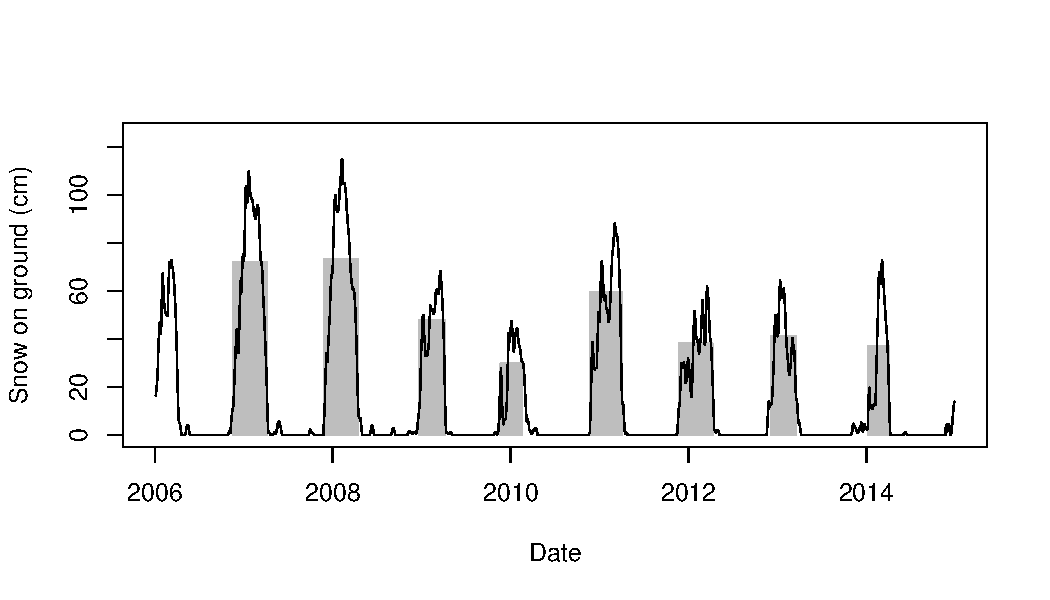
\includegraphics[width=1.0\textwidth]{report-barplots}
\vspace{-5mm}
\caption{{\footnotesize Average amount of snow over each winter season}}
\end{figure}

\end{frame}

\begin{frame}{Correlation}

\begin{itemize}
\item Average snow and temperature: --0.15
\item Peak and average snow: 0.96
\end{itemize}

\begin{table}[ht]
\begin{tabular}{c c c c}
\hline
Winter & Peak snow & Average snow & Average temperature \\ \hline
2006--2007 & 113 cm & 72 cm & -0.56 $^{\circ}$c \\
2007--2008 & 125 cm & 73 cm & -1.23 $^{\circ}$c \\
2008--2009 & 75 cm & 48 cm & -1.80 $^{\circ}$c \\
2009--2010 & 58 cm & 30 cm & -1.17 $^{\circ}$c \\
2010--2011 & 94 cm & 59 cm & -1.31 $^{\circ}$c \\
2011--2012 & 68 cm & 38 cm & -0.37 $^{\circ}$c \\
2012--2013 & 81 cm & 41 cm & -1.26 $^{\circ}$c \\
2013--2014 & 78 cm & 37 cm & -0.17 $^{\circ}$c \\ \hline
Average & 86 cm & 50 cm & -0.98 $^{\circ}$c \\ \hline
\end{tabular}
\caption{Snow and temperature measurements for winter seasons}
\end{table}

\end{frame}

\begin{frame}{Conclusion}

\section{Conclusion}

\begin{itemize}
\item Winter season starts Dec 3, ends Mar 26
\item Average snow present is 50 cm 
\item Snowfall downward trending
\item 2009--2010 was least severe winter 
\item Limitations
\begin{itemize}
\item No projections -- predictive ARIMA model could be used
\item Didn't account for wind, precipitation
\end{itemize}
\end{itemize}

\end{frame}

\end{document}